\documentclass{article}
\usepackage{authblk}
\usepackage[T1]{fontenc}
\usepackage{lmodern}
\usepackage{amsmath}
\usepackage{amssymb}
\usepackage[table,xcdraw]{xcolor}
\usepackage{physics}
\usepackage{siunitx}
\usepackage{float}
\usepackage{wrapfig}
\usepackage{sidecap}
\usepackage{color}
\usepackage{graphicx}
\usepackage{caption}
\usepackage{subcaption}
\usepackage{graphicx}
\usepackage{hyperref}
\usepackage[english]{babel}
\usepackage{multirow}
\usepackage{standalone}
\usepackage[toc,page]{appendix}
\usepackage{listings}
\usepackage{a4wide}
\usepackage{pdfpages}
\usepackage{float}
\usepackage[caption = false]{subfig}
\usepackage{mathtools}
\usepackage[normalem]{ulem}
\usepackage{arydshln}
\useunder{\uline}{\ul}{}
\usepackage[utf8]{inputenc}
\usepackage{relsize}
\usepackage{enumitem}
\usepackage{array}  % in your preamble
\usepackage[most]{tcolorbox}
\usepackage[table]{xcolor}
\numberwithin{equation}{section}
\numberwithin{equation}{subsection}

\title{Notes for Discrete Mathematics (2. Ed) by Rosen: Chapter 1: Logic and Proofs}
\author{Andreas Hansen}
\date{May 2025}

\begin{document}

\maketitle

\section*{\underline{Chapter 1.3: Propositional Equivalences} (pg. 26-37)}
\subsection*{Tautology and Contradiction: (pg. 26-27)}
\begin{center}
\noindent\fbox{
  \parbox{0.95\linewidth}{
    \textbf{Definition:} \textbf{Tautology}. A compound proposition that is always true, no matter what the truth values of the propositional
variables that occur in it, is called a tautology.
  }
}
\end{center}
\begin{center}
\noindent\fbox{
  \parbox{0.95\linewidth}{
    \textbf{Definition:} \textbf{Contradiction.} A compound proposition that is always
false is called a contradiction
  }
}
\end{center}
\begin{center}
\noindent\fbox{
  \parbox{0.95\linewidth}{
    \textbf{Definition:} \textbf{Contingency.} A compound proposition that is neither a tautology nor a contradiction
is called a contingency
  }
}
\end{center}

\begin{tcolorbox}[title=Example 1: Examples of tautologies and contradictions using just one propositional variable]
\textbf{Exercise:}  
\begin{center}
Consider the truth tables of $p\lor \neg p$ and $p \land \neg p$ 
\end{center}

\textbf{Strategy:}  
Remember the conjunction ($\land$) and disjunction ($\lor$) operators and write first truth and false for the propositional variable $p$ and then for its negation $\neg p$.

\vspace{5pt}
\textbf{Truth Table:}
\begin{center}
\rowcolors{2}{gray!10}{white}
\begin{tabular}{|c!{\vrule width 1pt}c|c!{\vrule width 1.5pt}c|c|}
\hline
\rowcolor{gray!20}
\textbf{$p$} & \textbf{$\neg p$} & \textbf{$p \lor \neg p$} & \textbf{$p \land \neg p$} \\
\hline
T & F & T & F \\
F & T & T & F \\
\hline
\end{tabular}
\end{center}

\vspace{5pt}
\textbf{Conclusion:}   \\
The compound proposition $p \lor \neg p$ is a \textbf{tautology} — always true. \\
The compound proposition $p \land \neg p$ is a \textbf{contradiction} — always false.
\end{tcolorbox}





\newpage
\subsection*{Logical Equivalences: (pg. 27-30)}
\vspace{5pt}
\tcbset{colback=gray!5, colframe=black!70, boxrule=0.5pt, arc=2pt, left=6pt, right=6pt, top=4pt, bottom=4pt}
\begin{tcolorbox}[title=Definition: Logically Equivalent]
The compound propositions $p$ and $q$ are called \textbf{logically equivalent} if 
\begin{center}
$p\leftrightarrow q$ is a tautology
\end{center}
The notation $p\equiv q $ denotes that $p$ and $q$ are logically equivalent.
\end{tcolorbox}
\begin{tcolorbox}[colback=white, colframe=gray!60, title=Remark 1]
The symbol $\equiv$ is not a logical connective, and $p\equiv q$ is not a compound proposition
but rather is the statement that $p\leftrightarrow q$ is a tautology. The symbol $\Leftrightarrow$ is sometimes used instead
of $\equiv$ to denote logical equivalence.
\end{tcolorbox}
\tcbset{colback=gray!5, colframe=black!70, boxrule=0.5pt, arc=2pt, left=6pt, right=6pt, top=4pt, bottom=4pt}
\begin{tcolorbox}[title=Definition: De Morgan’s Laws]
A pair of transformation rules, that state:
\begin{center}
$\neg (p\land q) \equiv \neg p \lor \neg q$ \\
$\neg (p\lor q) \equiv \neg p \land \neg q$
\end{center}

They can also be expressed as:

\begin{center}
\rowcolors{2}{gray!10}{white}
\begin{tabular}{|
    >{\centering\arraybackslash}m{3cm}  % centered vertically + horizontally
    |>{\centering\arraybackslash}m{2.5cm}  % centered vertically + horizontally
    |m{3.5cm}  %  column, vertically centered
    |m{3.5cm}|}  %  column, vertically centered
\hline
\rowcolor{gray!20}
\textbf{Logic} & \textbf{Boolean} & \textbf{English (simple)} & \textbf{English (formal)} \\
\hline
$\neg (p\land q) \equiv \neg p \lor \neg q$ & 
$\overline{p \land q} = \overline{p} \lor \overline{q}$  & The negation of "A and B" is the same as "not A or not B" & The complement of the union of two sets is the same as the intersection of their complements \\
\hline
$\neg (p\lor q) \equiv \neg p \land \neg q$ & $\overline{p \lor q} = \overline{p} \land \overline{q}$ & The negation of "A or B" is the same as "not A and not B" & The complement of the intersection of two sets is the same as the union of their complements\\
\hline  
\end{tabular}
\end{center}
\end{tcolorbox}

\begin{tcolorbox}[title=Example 1: Show 2. De Morgan´s Law with truth table]
\textbf{Exercise:}  
\begin{center}
Show that $\neg (p\lor q) $ and $\neg p \land \neg q$  are logically equivalent (using truth table) 
\end{center}
\textbf{Truth table:}
\begin{center}
\rowcolors{2}{gray!10}{white}
\begin{tabular}{|c|c!{\vrule width 1.5pt}c|c!{\vrule width 1.5pt}c|c|c|}
\hline
\rowcolor{gray!20}
$p$ & $q$ & $p \lor q$ & $\neg (p \lor q)$ & $\neg p$ & $\neg q$ & $\neg p \land \neg q$ \\
\hline
T & T & T & F & F & F & F \\
T & F & T & F & F & T & F \\
F & T & T & F & T & F & F \\
F & F & F & T & T & T & T \\
\hline
\end{tabular}    
\end{center}

\textbf{Conclusion:}  
Because the truth values of the compound propositions $\neg (p\lor q) $ and $\neg p \land \neg q$ agree for all possible combinations
of the truth values of $p$ and $q$, it follows that $\neg (p\lor q) \leftrightarrow \neg p \land \neg q$  is a tautology and
that these compound propositions are logically equivalent.
\end{tcolorbox}

\begin{tcolorbox}[title=Example 2: Show conditional-disjunction equivalence]
\textbf{Exercise:}  
\begin{center}
Show that $p\rightarrow q $ and $\neg p \lor q$  are logically equivalent (using truth table) 
\end{center}
\textbf{Truth table:}
\begin{center}
\rowcolors{2}{gray!10}{white}
\begin{tabular}{|c|c!{\vrule width 1.5pt}c|c|c|}
\hline
\rowcolor{gray!20}
$p$ & $q$ & $\neg p$ & $\neg p \lor q$ & $p \rightarrow q$ \\
\hline
T & T & T & F & F   \\
T & F & T & F & F   \\
F & T & T & F & T   \\
F & F & F & T & T   \\
\hline
\end{tabular}    
\end{center}

\textbf{Conclusion:}  
Because the truth values of the compound propositions $\neg (p\lor q) $ and $\neg p \land \neg q$ agree for all possible combinations
of the truth values of $p$ and $q$, it follows that $\neg (p\lor q) \leftrightarrow \neg p \land \neg q$  is a tautology and
that these compound propositions are logically equivalent.
\end{tcolorbox}
\begin{tcolorbox}[colback=white, colframe=gray!60, title=Remark 2]
If we establish a logical equivalence of two compound propositions involving three
different propositional variables $p$, $q$, and $r$. To use a truth table to establish such a logical
equivalence, we need eight rows, one for each possible combination of truth values of these
three variables. We symbolically represent these combinations by listing the truth values of $p$, $q$, and $r$, respectively.
\end{tcolorbox}
\begin{tcolorbox}[colback=white, colframe=gray!60, title=Remark 3]
These eight combinations of truth values are \textbf{TTT}, \textbf{TTF}, \textbf{TFT}, \textbf{TFF}, \textbf{FTT},
\textbf{FTF}, \textbf{FFT}, and \textbf{FFF}; we use this order when we display the rows of the truth table. Note that we
need to double the number of rows in the truth tableswe use to show that compound propositions
are equivalent for each additional propositional variable, so that 16 rows are needed to establish
the logical equivalence of two compound propositions involving four propositional variables,
and so on.
\end{tcolorbox}
\begin{tcolorbox}[colback=white, colframe=gray!60, title=Remark 4]
In general, $2^n$ rows are required if a compound proposition involves n propositional
variables. Because of the rapid growth of $2^n$, more efficient ways are needed to establish logical
equivalences, such as by using ones we already know
\end{tcolorbox}

\begin{tcolorbox}[title=Example 3: Distributive law
of disjunction over conjunction]
\textbf{Exercise:}  
\begin{center}
Show that $p\lor (q\land r) $ and $(p\lor q) \land (p \lor r)$  are logically equivalent (using truth table) 
\end{center}
\textbf{Truth table:}
\begin{center}
\rowcolors{2}{gray!10}{white}
\begin{tabular}{|c|c|c!{\vrule width 1.5pt}c|c!{\vrule width 1.5pt}c|c|c|}
\hline
\rowcolor{gray!20}
$p$ & $q$ & $r$ & $q \land r$ & $p \lor (q \land r)$ & $p \lor q$ & $p \lor r$ & $(p\lor q) \land (p\lor r)$ \\
\hline
T & T & T & T & T & T & T & T \\
\hline
T & T & F & F & T & T & T & T \\
\hline
T & F & T & F & T & T & T & T \\
\hline
T & F & F & F & T & T & T & T \\
\hline
F & T & T & T & T & T & T & T \\
\hline
F & T & F & F & F & T & F & F \\
\hline
F & F & T & F & F & T & F & F
\\
\hline
F & F & F & F & F & F & F & F \\ \hline
\end{tabular}    
\end{center}
\end{tcolorbox}

\begin{table}[h!]
\centering
\renewcommand{\arraystretch}{1.3} % Adjust vertical spacing
\rowcolors{2}{white}{gray!10} % Alternate: white, gray
\caption*{\textbf{Logical Equivalences: Logic, Programming, and Law Names}}
\begin{tabular}{|
    >{\centering\arraybackslash}m{5cm}
    |>{\centering\arraybackslash}m{7cm}
    |>{\centering\arraybackslash}m{4cm}|}
\hline
\rowcolor{gray!20}
\textbf{Equivalence (Logic)} & \textbf{Equivalence (Programming)} &\textbf{Name} \\
\hline
$p \lor \mathbf{F} \equiv p$ & p || false == p & Identity law (OR) \\
$p \land \mathbf{T} \equiv p$ & p \&\& true == p &Identity law (AND) \\
\hline
$p \lor \mathbf{T} \equiv \mathbf{T}$ & p || true == true & Domination law (OR) \\
$p \land \mathbf{F} \equiv \mathbf{F}$ & p \&\& false == false &  Domination law (AND) \\
\hline
$p \lor p \equiv p$ & p || p == p &  Idempotent law (OR) \\
$p \land p \equiv p$ & p \&\& p == p & Idempotent law (AND) \\
\hline
$\neg(\neg p) \equiv p$ & !!p == p & Double negation law \\
\hline
$p \lor q \equiv q \lor p$ & p || q == q || p & Commutative law (OR) \\
$p \land q \equiv q \land p$ & p \&\& q == q \&\& p & Commutative law (AND) \\
\hline
$(p \lor q) \lor r \equiv p \lor (q \lor r)$ & (p || q) || r == p || (q || r) & Associative law (OR) \\
$(p \land q) \land r \equiv p \land (q \land r)$ & (p \&\& q) \&\& r == p \&\& (q \&\& r) & Associative law (AND)  \\
\hline
$p \lor (q \land r) \equiv (p \lor q) \land (p \lor r)$ & p || (q \&\& r) == (p || q) \&\& (p || r)  & Distributive law (OR over AND) \\
$p \land (q \lor r) \equiv (p \land q) \lor (p \land r)$ & p \&\& (q || r) == (p \&\& q) || (p \&\& r) & Distributive law (AND over OR) \\
\hline
$\neg(p \land q) \equiv \neg p \lor \neg q$ & !(p \&\& q) == !p || !q &  De Morgan’s law (NOT AND $\rightarrow $ OR) \\
$\neg(p \lor q) \equiv \neg p \land \neg q$ & !(p || q) == !p \&\& !q & De Morgan’s law (NOT OR $\rightarrow$ AND) \\
\hline
$p \lor (p \land q) \equiv p$ & p || (p \&\& q) == p & Absorption law (OR) \\
$p \land (p \lor q) \equiv p$ & p \&\& (p || q) == p & Absorption law (AND) \\
\hline
$p \lor \neg p \equiv \mathbf{T}$ & p || !p == true   & Negation law (OR) \\
$p \land \neg p \equiv \mathbf{F}$ & p \&\& !p == false & Negation law (AND) \\
\hline
\end{tabular}
\end{table}

\newpage
\begin{table}[h!]
\centering
\renewcommand{\arraystretch}{1.3} % Adjust vertical spacing
\rowcolors{2}{white}{gray!10} % Alternate: white, gray
\caption*{\textbf{Logical Equivalences Involving Conditional Statements}}
\begin{tabular}{|
    >{\centering\arraybackslash}m{5cm}
    |>{\centering\arraybackslash}m{7cm}
    |>{\centering\arraybackslash}m{4cm}|}
\hline
\rowcolor{gray!20}
\textbf{Equivalence (Logic)} & \textbf{Equivalence (Programming)} &\textbf{Name} \\
\hline
$p \rightarrow q \equiv \neg p \lor q$ & !p || q & Conditional equivalence \\
\hline
$p \rightarrow q \equiv \neg q \rightarrow \neg p$ & !p || q == !q || !p & Contrapositive equivalence \\
\hline
$p \lor q \equiv \neg p \rightarrow q$ & !p || q & Implication from disjunction \\
\hline
$p \land q \equiv \neg(p \rightarrow \neg q)$ & !(p => !q) or !( !p || !q ) & Conjunction via implication \\
\hline
$\neg (p \rightarrow q) \equiv p \land \neg q$ & !( !p || q ) == p \&\& !q & Negation of implication \\
\hline
$(p\rightarrow q) \land (p \rightarrow r) \equiv p \rightarrow (q \land r)$ & (!p || q) \&\& (!p || r) == !p || (q \&\& r) & Distributive implication (AND) \\
\hline
$(p\rightarrow r) \land (q \rightarrow r) \equiv (p \lor q) \rightarrow r$ & (!p || r) \&\& (!q || r) == !(p || q) || r & Factoring implication (common result) \\
\hline
$(p\rightarrow q) \lor (p \rightarrow r) \equiv p \rightarrow (q \lor r)$ & (!p || q) || (!p || r) == !p || (q || r) & Distributive implication (OR) \\
\hline
$(p\rightarrow r) \lor (q \rightarrow r) \equiv (p \land q) \rightarrow r$ & (!p || r) || (!q || r) == !(p \&\& q) || r & Factoring implication (common antecedent) \\
\hline
\end{tabular}
\end{table}

\begin{table}[h!]
\centering
\renewcommand{\arraystretch}{1.3} % Adjust vertical spacing
\rowcolors{2}{white}{gray!10} % Alternate: white, gray
\caption*{\textbf{Logical
Equivalences Involving
Biconditional Statements}}
\begin{tabular}{|
    >{\centering\arraybackslash}m{5cm}
    |>{\centering\arraybackslash}m{5cm}
    |>{\centering\arraybackslash}m{6cm}|}
\hline
\rowcolor{gray!20}
\textbf{Equivalence (Logic)} & \textbf{Equivalence (Programming)} &\textbf{Name} \\
\hline
$p \leftrightarrow q \equiv (p \rightarrow q) \land (q \rightarrow p)$ &  (!p || q) \&\& (!q || p) & Biconditional as conjunction of implications   \\
\hline
$p \leftrightarrow q \equiv \neg q \leftrightarrow \neg p$ & !q == !p & Invariance under negation (logical symmetry)  \\
\hline
$p \leftrightarrow q \equiv (p \land q) \lor (\neg p \land \neg q)$ & (p \&\& q) || (!p \&\& !q) & Biconditional as agreement in truth value  \\
\hline
$\neg (p \leftrightarrow q) \equiv p \leftrightarrow \neg q$ & !(p == q) == (p == !q) & Negation of biconditional / XOR form \\
\hline
\end{tabular}
\end{table}


\begin{tcolorbox}[colback=white, colframe=gray!60, title=Remark 5]
The associative law for disjunction shows that the expression $p \lor q \lor r$ is well defined, in
the sense that it does not matter whether we first take the disjunction of $p$ with $q$ and then
the disjunction of $p\lor q$ with $r$, or if we first take the disjunction of $q$ and $r$ and then take the
disjunction of $p$ with $p \lor r$.
\end{tcolorbox}
\begin{tcolorbox}[colback=white, colframe=gray!60, title=Remark 6]
Similarly, the expression $p \land q \land r$ is well defined. By extending
this reasoning, it follows that $p_1 \lor p_2  \lor \ldots \lor p_n$ and $p_1 \land p_2 \land \ldots \land p_n$ are well defined whenever
$p_1, p_2,\ldots, p_n$ are propositions.
\end{tcolorbox}

\newpage
\begin{table}[h!]
\centering
\renewcommand{\arraystretch}{1.3} % Adjust vertical spacing
\rowcolors{2}{white}{gray!10} % Alternate: white, gray
\caption*{\textbf{Extended Version of De Morgan’s Laws}}
\begin{tabular}{|
    >{\centering\arraybackslash}m{7cm}
    |>{\centering\arraybackslash}m{4.5cm}
    |>{\centering\arraybackslash}m{5cm}|}
\hline
\rowcolor{gray!20}
\textbf{Explicit Form} & \textbf{Compact Form} & \textbf{Name} \\
\hline
$\neg(p_1 \lor p_2 \lor \ldots \lor p_n) \equiv \neg p_1 \land \neg p_2 \land \ldots \land \neg p_n$ 
& $ \neg \left(\bigvee_{j=1}^n p_j \right) \equiv \bigwedge_{j=1}^n \neg p_j $ 
& Generalized De Morgan’s Law (OR to AND) \\
\hline
$\neg(p_1 \land p_2 \land \ldots \land p_n) \equiv \neg p_1 \lor \neg p_2 \lor \ldots \lor \neg p_n$ 
& $ \neg \left(\bigwedge_{j=1}^n p_j \right) \equiv \bigvee_{j=1}^n \neg p_j $ 
& Generalized De Morgan’s Law (AND to OR) \\
\hline
\end{tabular}
\end{table}

\begin{tcolorbox}[colback=white, colframe=gray!60, title=Remark 7]
A truth table with $2^n$ rows is needed to prove the equivalence of two compound propositions
in $n$ variables. Note that the number of rows doubles for each additional propositional variable
added
\end{tcolorbox}
\begin{tcolorbox}[colback=white, colframe=gray!60, title=Remark 8]
Because $2^n$
grows extremely rapidly as $n$ increases , the use of truth tables to establish
equivalences becomes impractical as the number of variables grows. It is quicker to use other
methods, such as employing logical equivalences that we already know.
\end{tcolorbox}

\subsection*{Using De Morgan’s Laws (pg. 30)}
\begin{tcolorbox}[colback=white, colframe=gray!60, title=Remark 1]
When using De
Morgan’s laws,
remember to change
the logical connective
after you negate.
\end{tcolorbox}
\begin{tcolorbox}[colback=white, colframe=gray!60, title=Remark 2]
The two logical equivalences known as De Morgan’s laws are particularly important. They tell
us how to negate conjunctions and how to negate disjunctions.
\end{tcolorbox}
\begin{tcolorbox}[colback=white, colframe=gray!60, title=Remark 3]
In particular, the equivalence $\neg (p \lor q) \equiv \neg \land \neg q$ tells us that the negation of a disjunction is formed by taking the conjunction
of the negations of the component propositions.
\end{tcolorbox}
\begin{tcolorbox}[colback=white, colframe=gray!60, title=Remark 4]
Similarly, the equivalence $\neg (p \land q) \equiv \neg p \lor \neg q $
tells us that the negation of a conjunction is formed by taking the disjunction of the negations
of the component propositions.
\end{tcolorbox}

\begin{tcolorbox}[title=Example 1: Using De Morgan's Laws]
\textbf{Exercise:}  
\\ Use De Morgan’s laws to express the negations of:  
\begin{center}
\textit{“Miguel has a cellphone and he has a laptop computer”}  \\
\textit{“Heather will go to the concert or Steve will go to the concert”}    
\end{center}

\textbf{Let:}  
\begin{itemize}
    \item \textbf{p:} Miguel has a cellphone
    \item \textbf{q:} Miguel has a laptop computer
    \item \textbf{r:} Heather will go to the concert
    \item \textbf{s:} Steve will go to the concert
\end{itemize}

\textbf{Negation 1:}   
\begin{align*}
&\text{\textbf{Original}: } p \land q \quad \text{(Miguel has a cellphone and a laptop)} \\
&\text{\textbf{Negation}: } \neg(p \land q) \\
&\text{\textbf{Apply De Morgan's Law}: } \neg(p \land q) \equiv \neg p \lor \neg q \\
&\text{\textbf{English}: } \textit{Miguel does not have a cellphone or he does not have a laptop.}
\end{align*}
\textbf{Negation 2:}   
\begin{align*}
&\text{\textbf{Original}: } r \lor s \quad \text{(Heather or Steve will go to the concert)} \\
&\text{\textbf{Negation}: } \neg(r \lor s) \\
&\text{\textbf{Apply De Morgan's Law:} } \neg(r \lor s) \equiv \neg r \land \neg s \\
&\text{\textbf{English:} } \textit{Heather will not go to the concert and Steve will not go to the concert.}
\end{align*}
\end{tcolorbox}




\newpage
\subsection*{Constructing New Logical Equivalences (pg. 31-32)}
\begin{tcolorbox}[colback=white, colframe=gray!60, title=Remark 1]
We use the fact that if $p$ and $q$ are logically equivalent and $q$ and $r$ are logically equivalent, then $p$ and $r$ are
logically equivalent (See Exercise 60)
\end{tcolorbox}

\begin{tcolorbox}[title=Example 1: Construct new logical equivalence]
\textbf{Exercise:}  
\\ Show the logical equivalence: 
\begin{center}
$\neg (p\rightarrow q) \equiv p \land \neg q$  
\end{center}

\textbf{Strategy:}  \\
We will establish this equivalence by developing a
series of logical equivalences, using one of the equivalences from our previous tables, starting with
$\neg (p\rightarrow q) $ and ending with $p \land \neg q$   \\ \\
\textbf{Using logical equivalences:}   
\begin{align*}
\neg (p\rightarrow q) &\equiv \neg (\neg p \lor q)  \ \ \ (\textbf{conditional-disjunction equivalence, pg. 3, example 2}) \\
&\equiv \neg (\neg p) \land \neg q \ \ \ \textbf{(second De Morgan law, pg. 4)} \\
&\equiv p\land \neg q \ \ \ \textbf{(double negation law, pg. 4)} \\
\end{align*}
\end{tcolorbox}

\begin{tcolorbox}[title=Example 2: Construct new logical equivalence]
\textbf{Exercise:}  
\\ Show the logical equivalence: 
\begin{center}
$\neg (p \lor (\neg p\land q)) \equiv \neg p \land \neg q$
\end{center}

\textbf{Strategy:}  \\
We will establish this equivalence by developing a
series of logical equivalences, using one of the equivalences from our previous tables, starting with
$\neg (p \lor (\neg p\land q))$ and ending with $\neg p \land \neg q$ \\ \\
\textbf{Using logical equivalences:}   
\begin{align*}
\neg (p \lor (\neg p\land q)) &\equiv \neg p \land \neg (\neg p\land q) \ \ \ \textbf{(second De Morgan law, pg. 4)} \\
&\equiv \neg p \land (\neg (\neg p)\lor  \neg q)) \ \ \ \textbf{(first De Morgan law, pg. 4)} \\
&\equiv\neg p \land (p \lor \neg q) \ \ \ \textbf{(double negation law, pg. 4)} \\
&\equiv (\neg p \land p) \lor (\neg p \land \neg q) \ \ \ \textbf{(distributive law (AND over OR), pg. 4)} \\
&\equiv \mathbf{F} \lor (\neg p \land \neg q) \ \ \ \textbf{(negation law (AND), pg. 4)} \\
&\equiv (\neg p \land \neg q) \lor \mathbf{F}  \ \ \ \textbf{(commutative law (OR), pg. 4)} \\
&\equiv \neg p \land \neg q  \ \ \ \textbf{(identity law (OR), pg. 4)} \\
\end{align*}
\end{tcolorbox}

\begin{tcolorbox}[title=Example 3: Construct tautology]
\textbf{Exercise:}  
\\ Show the tautology: 
\begin{center}
$(p\land q) \rightarrow (p\lor q)$
\end{center}

\textbf{Strategy:}  \\
To show that this statement is a tautology, we will use logical equivalences to demonstrate
that it is logically equivalent to \textbf{T}. \\ \\
\textbf{Using logical equivalences:}   
\begin{align*}
(p\land q) \rightarrow (p\lor q) &\equiv \neg (p \land q) \lor (p \lor q) \ \  (\textbf{conditional-disjunction equivalence, pg. 3, ex. 2}) \\
&\equiv (\neg p \lor   \neg q) \lor (p \lor q) \ \ \ \textbf{(first De Morgan law, pg. 4)} \\
&\equiv (\neg p \lor p) \lor (\neg q \lor q)
\ \ \ \textbf{(associative + commutative (OR) laws, pg. 4)} \\
&\equiv \mathbf{T} \lor \mathbf{T} \ \ \ \textbf{(tautology, pg. 1, ex. 1 + commutative (OR) law, pg. 4) } \\
&\equiv \mathbf{T} \ \ \ \textbf{(domination law, pg. 4,) } 
\end{align*}
\end{tcolorbox}
\subsection*{Satisfiability (pg. 33)}
\begin{center}
\noindent\fbox{
  \parbox{0.95\linewidth}{
    \textbf{Definition:} \textbf{Satisfiable}. A compound proposition is satisfiable if there is an assignment of truth values to its variables
that makes it true (that is, when it is a tautology or a contingency).
  }
}
\end{center}
\begin{center}
\noindent\fbox{
  \parbox{0.95\linewidth}{
    \textbf{Definition:} \textbf{Unsatisfiable}. 
When no such assignments
exists, that is, when the compound proposition is false for all assignments of truth values to
its variables, the compound proposition is unsatisfiable.
  }
}
\end{center}

\begin{tcolorbox}[colback=white, colframe=gray!60, title=Remark 1]
Note that a compound proposition is
unsatisfiable if and only if its negation is true for all assignments of truth values to the variables,
that is, if and only if its negation is a tautology.
\end{tcolorbox}
\begin{tcolorbox}[colback=white, colframe=gray!60, title=Remark 2]
When we find a particular assignment of truth values that makes a compound proposition
true,we have shown that it is satisfiable; such an assignment is called a \textbf{solution} of this particular
satisfiability problem.
\end{tcolorbox}
\begin{tcolorbox}[colback=white, colframe=gray!60, title=Remark 3]
However, to show that a compound proposition is unsatisfiable, we need
to show that every assignment of truth values to its variables makes it false. Although we can
always use a truth table to determine whether a compound proposition is satisfiable, it is often
more efficient not to.
\end{tcolorbox}

\newpage
\begin{tcolorbox}[title=Example 1: Satisfiable compound propositions]
\textbf{Exercise:}  
\\ Determine whether each of the compound propositions is satisfiable
\begin{center}
$(p\lor \neg q) \land (q \lor \neg r) \land (r \lor \neg p)$ \\ 
$(p\lor q \lor r) \land (\neg p \lor \neg q \lor \neg r)$
\\
$(p\lor \neg q) \land (q \lor \neg r) \land (r \lor \neg p) \land (p \lor q \lor r) \land (\neg p \lor \neg q \lor \neg r)$
\end{center}

\textbf{Strategy:}  \\
Instead of using a truth table to solve this problem, we will reason about truth values. \\ \\
\textbf{First compound proposition:} \\
We have $(p\lor \neg q) \land (q \lor \neg r) \land (r \lor \neg p)$ is true when the three variables $p$, $q$, and $r$ have the same truth value.
Hence, it is satisfiable as there is at least
one assignment of truth values for $p$, $q$, and $r$ that makes it true.
\\ \\
\textbf{Second compound proposition:} \\
Similarly, note that $(p\lor q \lor r) \land (\neg p \lor \neg q \lor \neg r)$ is true when at least one of $p$, $q$, and $r$ is true and at least one is false. Hence, $(p\lor q \lor r) \land (\neg p \lor \neg q \lor \neg r)$ is satisfiable, as there is at least
one assignment of truth values for $p$, $q$, and $r$ that makes it true. \\ \\
\textbf{Third compound proposition:} \\
Finally, note that for $(p\lor \neg q) \land (q \lor \neg r) \land (r \lor \neg p) \land (p \lor q \lor r) \land (\neg p \lor \neg q \lor \neg r)$ to be true:
\\ \\ Both: 
\begin{center}
$(p\lor \neg q) \land (q \lor \neg r) \land (r \lor \neg p)$    
\end{center}
and 
\begin{center}
 $(p \lor q \lor r) \land (\neg p \lor \neg q \lor \neg r)$   
\end{center}
must both be true. 
\\ For the first to be true, $(p\lor \neg q) \land (q \lor \neg r) \land (r \lor \neg p)$ ,  the three variables must have the same truth values. \\
For the second to be true, $(p \lor q \lor r) \land (\neg p \lor \neg q \lor \neg r)$ at least one of the three variables must be true and at least one must be
false. \\ \\
However, these conditions are contradictory. From these observations we conclude
that no assignment of truth values to $p$, $q$, and $r$ makes $(p\lor \neg q) \land (q \lor \neg r) \land (r \lor \neg p) \land (p \lor q \lor r) \land (\neg p \lor \neg q \lor \neg r)$ true. Hence, it is unsatisfiable.
\end{tcolorbox}










¨.
\newpage
\subsection*{Applications of Satisfiability (pg. 33-37)}
\begin{tcolorbox}[title=Example 1: The n-Queens Problem (1/2)]
\textbf{Exercise:}  
\\ The n-queens problem asks for a placement of $n$ queens on an n × n
chessboard so that no queen can attack another queen. This means that no two queens can be
placed in the same row, in the same column, or on the same diagonal. We display a solution
to the eight-queens problem below.

\centering
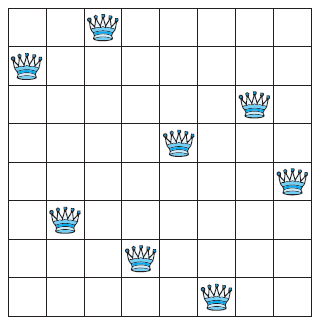
\includegraphics[width=0.3\linewidth]{chp1_3_propequiv/n_queens.png}

\raggedright
\textbf{Strategy:} \newline 
To model the n-queens problem as a satisfiability problem, we introduce $n^2$ variables, $p(i,j)$ for $i = 1,2, \ldots, n$ and $j = 1,2, \ldots, n$.
\newline For a given placement of a queens on the chessboard:
\begin{center}
$p(i, j)$ is \textbf{true} when there is a queen on the square in the i'th row and j'th column. \newline and \textbf{false} otherwise.
\end{center}
Note that squares $(i,j)$ and $(i', j')$ are on the same diagonal if either:
\begin{center}
$i+ i' = j+ j'$ \ \ or \ \ $i-i' = j - j'$    
\end{center}
\textbf{Implementing solution:} \newline
\textbf{Step 1:}
For no two of the $n$ queens to be in the same row, there must be one queen in each row. We
can show that there is one queen in each row by verifying that every row contains at least one
queen and that every row contains at most one queen. 
\begin{center}
$\bigvee_{j=1}^{n} p(i,j)$ asserts that
row $i$ contains at least one queen \newline
$Q_1 = \bigwedge_{i=1}^{n} \bigvee_{j=1}^{n} p(i,j)$ \textbf{asserts that every row contains at least one queen}
\end{center}
\textbf{Step 2:} For every row to include at most one queen, it must be the case that $p(i, j)$ and $p(k, j)$ are
not both true for integers $j$ and $k$ with $1 \leq j < k \leq n$. \newline
Observe that $\neg p(i,j) \lor \neg p(i,k)$ asserts that at least one of $\neg p(i,j)$ and $\neg p(i,k)$  is true, which means that at least one of $p(i, j)$ and $p(i, k)$ is false.
So, to check that there is: 
\begin{center}
$Q_2 = \bigwedge_{i=1}^n \bigwedge_{j=1}^{n-1} \bigwedge_{k=j+1}^{n} (\neg p(i,j) \lor \neg p(k,j)) $    \ \textbf{asserts at most one queen in each row}
\end{center}
\textbf{Step 3:} We have do the same, but for coloumns:
\begin{center}
$Q_3 = \bigwedge_{i=1}^n \bigwedge_{j=1}^{n-1} \bigwedge_{k=i+1}^{n} (\neg p(i,j) \lor \neg p(k,j)) $     \textbf{no column contains more than one queen}
\end{center}   
\end{tcolorbox}

\newpage
\begin{tcolorbox}[title=Example 1: The n-Queens Problem (2/2)]
\textbf{Step 4:} Now we consider the diagonals, and we have to make sure, that no diagonal contains two queens. We will first look at the main diagonal, which are characterized by having constant values of $i-j$. So we have to enforce that for all cells ($i,j$) there is no other queen on $(i+k, j+k)$, where $k$ increases along the diagonal:
\begin{center}
$Q_4 = \bigwedge_{i=1}^{n-1} \bigwedge_{j=1}^{n-1} \bigwedge_{k=1}^{min(n-i,n-j)} (\neg p(i,j) \lor \neg p(i+k,j+k)) $   \ \  \textbf{Main diagonal}
\end{center} 
\textbf{Step 5:} These anti-diagonals are characterized by constant values of $i+j$. So we have to enforce that for all cells ($i,j$) there is no other queen on $(i+k, j-k)$, where $k$ increases along the diagonal: 
\begin{center}
$Q_5 = \bigwedge_{i=1}^{n-1} \bigwedge_{j=2}^{n} \bigwedge_{k=1}^{min(n-i,j-1)} (\neg p(i,j) \lor \neg p(i+k,j-k)) $  \ \  \textbf{Anti-diagonal} 
\end{center} 
\textbf{Step 6:} Putting all this together, we find that the solutions of the n-queens problem are given
by the assignments of truth values to the variables $p(i,j) $ 
\begin{center}
$i=1,2,\ldots,n$  and $j=1,2,\ldots,n$ that make the following true
\end{center}
\begin{center}
$Q=Q_1 \land Q_2 \land Q_3 \land Q_4 \land Q_5$    
\end{center}{}
\end{tcolorbox}


\begin{tcolorbox}[title=Example 2: Sudoku puzzles (1/2)]
\textbf{Exercise:} \newline
Sudoku puzzles are constructed using a 9 × 9 grid made up of nine 3 × 3 subgrids, known as blocks \newline
For each puzzle, some of the 81 cells, called givens,
are assigned one of the numbers 1, 2,…, 9, and the other cells are blank. The puzzle is solved
by assigning a number to each blank cell so that every row, every column, and every one of the
nine 3 × 3 blocks contains each of the nine possible numbers.
\newline Note that instead of using a 9 × 9
grid, Sudoku puzzles can be based on $n^2 \times n^2$ grids, for any positive integer n, with the $n^2 \times n^2$ 
grid made up of $n^2$ $n \times n$  subgrids.
\newline \newline
\textbf{Strategy:} \newline 
To encode a Sudoku puzzle, let $p(i, j, n)$ denote the proposition that is true when the number
n is in the cell in the i'th row and j'th column. There are 9 × 9 × 9 = 729 such propositions, as i,
j, and n all range from 1 to 9. For example, for the puzzle in Figure 2, the number 6 is given as
the value in the fifth row and first column. Hence, we see that $p(5, 1, 6)$ is true, but $p(5, j, 6)$ is
false for $j = 2, 3,\ldots, 9$.
\newline 
\newline
Given a particular Sudoku puzzle, we begin by encoding each of the given values. Then,
we construct compound propositions that assert that every row contains every number, every
column contains every number, every 3 × 3 block contains every number, and each cell contains
no more than one number. \newline It follows, as the reader should verify, that the Sudoku puzzle is solved
by finding an assignment of truth values to the 729 propositions $p(i, j, n)$ with $i$, $j$, and $n$ each
ranging from 1 to 9 that makes the conjunction of all these compound propositions true. \newline After
listing these assertions, we will explain how to construct the assertion that every row contains
every integer from 1 to 9. \newline We will leave the construction of the other assertions that every
column contains every number and each of the nine 3 × 3 blocks contains every number to the
exercises
\end{tcolorbox}

\newpage
\begin{tcolorbox}[title=Example 2: Sudoku puzzles (2/2)]
\textbf{Solution:} \newline
\textbf{Step 1:} \newline
For each cell with a given value, we assert $p(i, j, n)$ when the cell in row $i$ and column $j$
has the given value $n$.
\newline \textbf{Step 2:} \newline
First, to \textbf{assert that row $i$ contains the number $n$}, we form
\begin{center}
$\bigvee_{j=1}^9 p(i,j,n)$    
\end{center}
\textbf{Step 3:}
\newline
To assert that\textbf{ row $i$ contains all $n$ numbers}, we form the conjunction of these disjunctions over all nine possible values of $n$, giving us
\begin{center}
$\bigwedge_{n=1}^9 \bigvee_{j=1}^9 p(i,j,n)$    
\end{center}
\textbf{Step 4:}
\newline
Finally, to \textbf{assert that every row contains  every number}, we take the conjunction
\begin{center}
$\bigwedge_{i=1}^9 \bigwedge_{n=1}^9 \bigvee_{j=1}^9 p(i,j,n)$    
\end{center}
\textbf{Step 5:}
\newline
(Exercises 71 and 72 ask for explanations of the assertions
that every column contains every number and that each of the nine 3 × 3 blocks contains
every number.)
\begin{center}
$\bigwedge_{j=1}^9 \bigwedge_{n=1}^9 \bigvee_{i=1}^9 p(i,j,n)$ \ \ \ \textbf{assert that every column contains every number}  \newline \newline
And that \textbf{assert that each of the nine 3 × 3 blocks contains every number;}
$\bigwedge_{r=0}^2 \bigwedge_{s=0}^2 \bigwedge_{n=1}^9 \bigvee_{i=1}^3 \bigvee_{j=1}^3 p(3r+i,3s+j,n)  $
\end{center}

\end{tcolorbox}





\newpage
\subsection*{Solving Satisfiability Problems (pg. 37)}
\begin{tcolorbox}[colback=white, colframe=gray!60, title=Remark 1]
A \textbf{truth table} can be used to determine whether a compound proposition is \textbf{satisfiable}, or
equivalently, whether its negation is a tautology (see \textbf{Exercise 64}). \newline
This can be done by
hand for a compound proposition with a small number of variables, but when the number
of variables grows, this becomes impractical.
\end{tcolorbox}
\begin{tcolorbox}[colback=white, colframe=gray!60, title=Remark 2]
\textbf{Because the problem scales as $2^n$, where $n$ is the number of variables.} \newline
For instance, there are $2^{20} = 1,048,576 \ \text{rows}$
in the truth table for a compound proposition with 20 variables. Thus, you need a computer
to help you determine, in this way, whether a compound proposition in 20 variables is
satisfiable.
\end{tcolorbox}
\begin{tcolorbox}[colback=white, colframe=gray!60, title=Remark 3]
When many applications are modeled, questions concerning the satisfiability of compound
propositions with hundreds, thousands, or millions of variables arise. Note, for example, that
when there are 1000 variables, checking every one of the $2^{1000}$ (a number with more than 300
decimal digits) possible combinations of truth values of the variables in a compound proposition
cannot be done by a computer in even trillions of years
\end{tcolorbox}
\begin{tcolorbox}[colback=white, colframe=gray!60, title=Remark 4]
No procedure is known that a computer
can follow to determine in a reasonable amount of time whether an arbitrary compound
proposition in such a large number of variables is satisfiable. However, progress has been made
developing methods for solving the satisfiability problem for the particular types of compound
propositions that arise in practical applications, such as for the solution of Sudoku puzzles.
\end{tcolorbox}
\begin{tcolorbox}[colback=white, colframe=gray!60, title=Remark 5]
Many computer programs have been developed for solving satisfiability problems which have
practical use. \newline In our discussion of the subject of algorithms in Chapter 3, we will discuss this
question further. In particular, we will explain the important role \textbf{the propositional satisfiability
problem plays in the study of the complexity of algorithms}
\end{tcolorbox}







\end{document}
